\documentclass[a4paper]{article}

\usepackage[portuguese]{babel}
\usepackage[utf8]{inputenc}
\usepackage{indentfirst}
\usepackage{graphicx}
\usepackage{verbatim}
\usepackage{caption}
\usepackage{subcaption}
\usepackage{wrapfig}
\usepackage{ragged2e}
\usepackage{listings}
\usepackage{float}

\begin{document}

\setlength{\textwidth}{16cm}
\setlength{\textheight}{22cm}

\title{\Huge\textbf{Eximo - LAIG3}\linebreak\linebreak\linebreak
\Large\textbf{Manual de Utilizador}\linebreak\linebreak
\linebreak\linebreak

\includegraphics[scale=0.1]{res/feup-logo.png}\linebreak\linebreak
\linebreak\linebreak
\Large{Mestrado Integrado em Engenharia Informática e Computação} \linebreak\linebreak
\Large{Laboratório de Aplicações com Interface Gráfica}\linebreak
}

\author{\textbf{T6G10: Eximo}\\
Henrique Manuel Martins Ferrolho -  201202772\\
João Filipe Figueiredo Pereira - 201104203 \\
Maria João Pombinho Miranda - 201204026 \\
\linebreak\linebreak \\
 \\ Faculdade de Engenharia da Universidade do Porto \\ Rua Roberto Frias, s\/n, 4200-465 Porto, Portugal \linebreak\linebreak\linebreak
\linebreak\linebreak\vspace{1cm}}

\maketitle
\thispagestyle{empty}

%************************************************************************************************
%************************************************************************************************

\newpage

%Todas as figuras devem ser referidas no texto. %\ref{fig:codigoFigura}
%
%%Exemplo de código para inserção de figuras
%%\begin{figure}[h!]
%%\begin{center}
%%\includegraphics[height=1.5cm,width=1.5cm]{white_piece.png}
%%\caption{Peça Branca - Jogador 1}
%%\label{fig:1}
%%\end{center}
%%\end{figure}
%%\includegraphics[scale=0.5]{path relativo da imagem}
%%\includegraphics[scale=•]{•} relativo da imagem}

%%\begin{figure}[h!]
%%\centering
%%\includegraphics[height=1.5cm,width=1.5cm]{white_piece.png}
%%\caption{Peça Branca}
%%\label{fig:whitePiece}
%%\end{figure}

%%\hfill

%%\begin{figure}[h!]
%%\centering
%%
\includegraphics[height=1.5cm,width=1.5cm]{black_piece.png}
%%\caption{Peça Preta}
%%\label{fig:blackPiece}
%%\end{figure}

%%\hfill

%%\begin{figure}[h!]
%%\centering
%%\includegraphics[height=3cm,width=3cm]{board.png}
%%\caption{Tabuleiro}
%%\label{fig:board}
%%\end{figure}




%
%
%\textit{Para escrever em itálico}
%\textbf{Para escrever em negrito}
%Para escrever em letra normal
%``Para escrever texto entre aspas''
%
%Para fazer parágrafo, deixar uma linha em branco.
%
%Como fazer bullet points:
%\begin{itemize}
	%\item Item1
	%\item Item2
%\end{itemize}
%
%Como enumerar itens:
%\begin{enumerate}
	%\item Item 1
	%\item Item 2
%\end{enumerate}
%
%\begin{quote}``Isto é uma citação''\end{quote}

\newpage

%%%%%%%%%%%%%%%%%%%%%%%%%%
\section{O Jogo Eximo}
%%Descrever detalhadamente o jogo, a sua história e, principalmente, as suas regras.
%%Devem ser incluidas imagens apropriadas para explicar o funcionamento do jogo.
%%Devem ser incluidas as fontes de informação (e.g. URLs em rodapé).

\large{\textbf{História}}
\begin{small}

Eximo é um jogo de tabuleiro da família das Damas, concebido em 1 de Fevereiro de 2013.\newline
\end{small}

\large{\textbf{Detalhes do Jogo}}
\begin{small}

O jogo realiza-se num tabuleiro de dimensões 8x8, em que as casas têm todas cores semelhantes. Cada jogador começa com 16 peças colocadas em locais pré-definidos no respectivo lado do tabuleiro, como mostra a imagem abaixo.\newline

\begin{figure}[h!]
  \begin{minipage}[h!]{0.2\textwidth}
    \includegraphics[width=0.4\textwidth]{res/white_piece.png}
    \centering
    \caption{Peça branca}
    \label{fig:2}
  \end{minipage}
	\quad\quad\quad
  \begin{minipage}[h!]{0.2\textwidth}
    \includegraphics[width=\textwidth]{res/board.png}
    \caption{Tabuleiro}
    \label{fig:3}
  \end{minipage}
	\quad\quad\quad
  \begin{minipage}[h!]{0.2\textwidth}
    
\includegraphics[width=0.4\textwidth]{res/black_piece.png}
	\centering
    \caption{Peça preta}
    \label{fig:4}
  \end{minipage}
\end{figure}

No jogo, as movimentações e as capturas podem ser ortogonais ou diagonais. Há apenas um tipo de peça: os homens. Os homens podem saltar sem efectuar captura. Quando um homem atinge a última linha, ocorre a libertação de outro homem.
\end{small}\newline

\large{\textbf{Objectivo}}
\begin{small}

O objectivo do jogo é, tal como nas Damas, \textbf{capturar todas as peças} do oponente, saltando sobre elas, ou \textbf{incapacitar o adversário} de realizar qualquer movimento.
\end{small}\newline

\large{\textbf{Jogada}}
\begin{small}

Em cada jogada, um jogador pode fazer uma de duas acções: \textbf{mover ou capturar}.
\end{small}\newline

\large{\textbf{Movimento}}
\begin{small}

Uma peça pode mover-se em três direcções: para a frente ou na diagonal (\textbf{norte, nordeste ou noroeste}). Numa jogada, o movimento nunca pode ser efectuado para a retaguarda. 

Existem dois tipos de movimentos: \textbf{Normal e Salto}. 
\begin{itemize}
\item \textbf{Movimento Normal}:
uma peça move-se para uma \textbf{casa adjacente e vazia}. 
\item \textbf{Movimento em Salto}:
\textbf{uma peça salta sobre uma peça aliada adjacente, se e só se a casa correspondente} (ao lado da peça aliada) \textbf{estiver vazia}, colocando assim a peça nessa casa. Se a mesma peça do jogador puder continuar a realizar o mesmo movimento de salto sobre outra peça amigável então terá de o fazer. \textbf{Durante um movimento de salto a peça não pode capturar peças inimigas}.

Quando existe \textbf{mais do que uma forma de saltar}, o jogador \textbf{pode escolher a peça que irá usar para executar o salto}, bem como o tipo de salto ou sequência de saltos a fazer. Não é obrigatório que a sequência de saltos escolhida pelo jogador seja aquela que possui o maior número de saltos; porém, \textbf{após escolher uma sequência, o jogador deve executar todos os saltos possíveis}.
\end{itemize}
\end{small}

\begin{figure}[h!]
  \begin{minipage}[h!]{0.3\textwidth}
    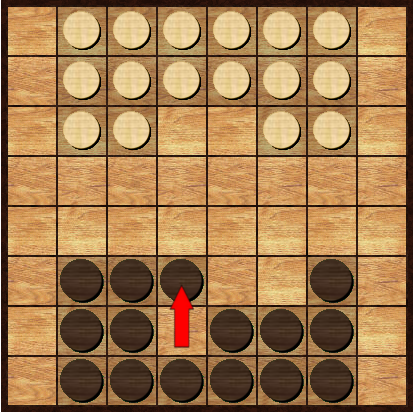
\includegraphics[width=\textwidth]{res/normalMove.png}
    \caption{Movimento Normal}
    \label{fig:5}
  \end{minipage}
\quad\quad\quad\quad\quad\quad\quad\quad
  \begin{minipage}[h!]{0.3\textwidth}
    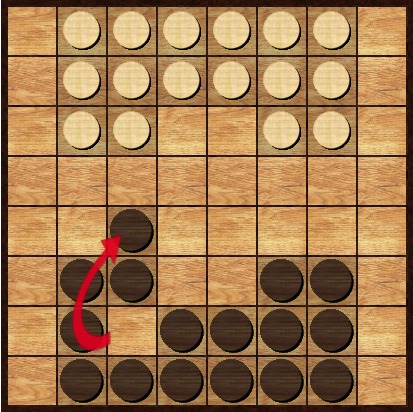
\includegraphics[width=\textwidth]{res/jumpMove.png}
    \caption{Movimento em Salto}
    \label{fig:6}
  \end{minipage}
  \caption{Movimentos}
\end{figure}

\large{\textbf{Captura}}
\begin{small}

Um \textbf{jogador pode capturar} em cinco direcções: \textbf{frente}, \textbf{diagonal para a frente}, \textbf{direita} ou \textbf{esquerda} (norte, nordeste, noroeste, este ou oeste). 

\begin{itemize}
\item \textbf{Captura}:
um jogador \textbf{salta sobre uma peça adjacente do adversário}, se a \textbf{próxima casa}, na mesma direcção, \textbf{estiver vazia}, colocando, assim, a peça sobre essa casa. A \textbf{peça do oponente é removida do tabuleiro}. Se a \textbf{peça} do mesmo jogador \textbf{puder continuar a capturar outras peças do adversário}, então \textbf{deve fazê-lo}. A \textbf{captura é obrigatória} e deve continuar enquanto for possível.
\end{itemize}

\begin{figure}[h!]
  \begin{minipage}[h!]{0.3\textwidth}
    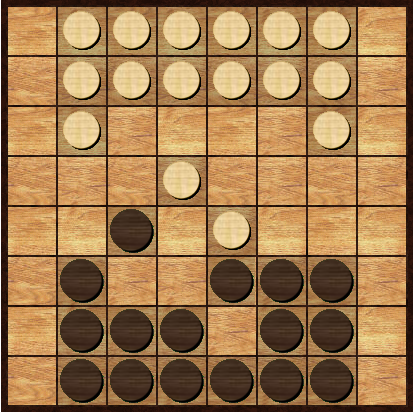
\includegraphics[height=5cm,width=5cm]{res/captureMove.png}
    \caption{Estado anterior à captura}
    \label{fig:7}
  \end{minipage}
	\quad\quad\quad\quad\quad\quad\quad
  \begin{minipage}[h!]{0.3\textwidth}
    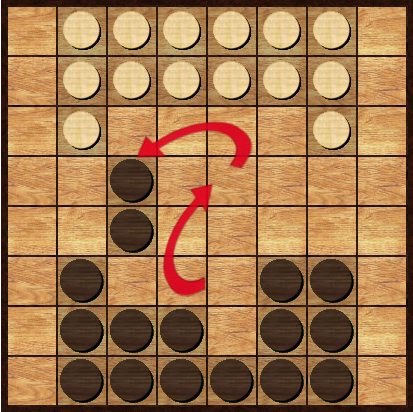
\includegraphics[height=5cm,width=5cm]{res/captureMoveResult.png}
    \caption{Estado posterior à captura}
    \label{fig:8}
  \end{minipage}
\end{figure}

Tal como no \textbf{Movimento de Salto}, \textbf{o jogador escolhe} livremente \textbf{qual a sequência de saltos a efectuar}.
\end{small}\newline

\large{\textbf{Última Linha}}
\begin{small}

Quando uma peça atinge a extremidade do tabuleiro, essa peça é removida de imediato e o jogador recebe dois movimentos extra para efectuar nesse mesmo momento: colocar duas peças novas numa casa vazia localizada nas duas primeiras linhas, à excepção das quatro casas laterais (duas do lado esquerdo, e duas do lado direito).
\end{small}\newline


\section{Compilação do Programa}
\large{\textbf{Eximo - PROLOG}}

\begin{small}
Antes de tudo, é necessária a instalação do Sicstus para executar o programa desenvolvido em PROLOG. Tendo este passo realizado, abrimos um terminal onde consultamos o ficheiro \textbf{server.pl} da seguinte forma:

\textbf{\textit{consult('caminho-para-o-ficheiro').}}

seguido da sua execução:

\textbf{\textit{server.}}

Neste ponto o programa já se encontra à espera de uma resposta para ligação com outro.

\hfill
\end{small}

\large{\textbf{Eximo - C++/OpenGL}}

\begin{small}
Para executar a aplicação desenvolvida em C++ basta correr o executável com o ficheiro .XML já presente.

\textbf{\textit{./LAIG3 "caminho-para-o-ficheiro-eximo.xml"}}

A conexão é deste modo feita, estando o programa a correr normalmente. Para a aplicação das texturas é necessário a pasta das mesmas estar junto ao executável.
\end{small}

\section{Interação do Utilizador}

\begin{small}
O jogo Eximo disponibiliza diversas funcionalidades ao utilizador, destacando-se os movimentos, a escolha das câmaras e do tema a aplicar ao jogo, e o possível controlo de jogadas.

Para realizar movimentações seleciona-se, com o botão esquerdo do rato, a célula com a peça a movimentar, e de seguida seleciona-se a célula de destino. Para cancelar a seleção de uma célula de origem basta clicar no botão direito do rato.

Apresenta-se de seguida os painéis contendo as funcionalidades do jogo.
\begin{figure}[h!]
   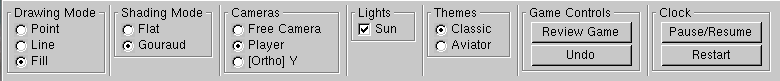
\includegraphics[width=0.8\textwidth]{res/gameControls.png}
   \caption{Controlos de jogo}
   \label{fig:9}
\end{figure}

No menu \textbf{Cameras} estão disponivéis três tipos de câmara:

	- \textit{Free Camera}, permite ao utilizador explorar com total liberdade o cenário de jogo;
	
	- \textit{Player}, é a câmara de jogo. Esta câmara roda à volta do tabuleiro, jogada a jogada.

	- \textit{[Ortho] Y} é uma câmara que se posiciona em cima do tabuleiro. Esta câmara é estática e não é permitido ao utilizador mudar a sua posição.
	

No menu \textbf{Themes} é permitido ao utilizador escolher o tema com o qual prefere jogar. Entre os temas existe o \textit{Classic} que representa os tabuleiros originais feitos em madeira e com peças normais; o segundo, \textit{Aviator}, que muda o ambiente de jogo para tons metálicos e as suas peças para aviões.

No menu \textbf{Game Controls} existem dois botões; \textit{Review Game}, que reproduz o filme de jogo ocorrido até ao momento, e \textit{Undo} para o utilizador cancelar a jogada realizada previemente.

No menu \textbf{Clock} é possível ao utilizador pausar e recomeçar o tempo de jogo, com \textit{Pause/Resume} ou reiniciá-lo através de \textit{Restart}.



\end{small}
\end{document}
